% ============================================================
%  深圳大学实验报告模板(SZU Experiment Report Template)
% This template can be modified according to the specific requirements of your experiment or project.
% Produced by: Chao Fan and Kewei Ou, AI School of SZU
% ============================================================

\documentclass[a4paper,12pt]{article}

% ----------------------------
% 中文与字体支持
% ----------------------------
\usepackage{fontspec}    % 字体支持
\usepackage{xeCJK}       % 中文字体支持
\setCJKmainfont{Noto Serif CJK SC} % 设置中文字体(Overleaf自带Noto字体)

% ----------------------------
% 页面设置与常用宏包
% ----------------------------
\usepackage{geometry}    % 页面边距控制
\geometry{left=1in, right=1in, top=1in, bottom=1in}

\usepackage{longtable}   % 支持长表格
\usepackage{graphicx}    % 插入图片
\usepackage{fancyhdr}    % 页眉页脚控制
\usepackage{tikz}        % 绘制框线等图形
\usetikzlibrary{calc}    % 坐标计算
\usepackage{verbatim}    % 显示代码块
\usepackage{float}       % 控制图片浮动位置([H]参数)
\usepackage{subcaption}

% ----------------------------
% 页眉页脚设置
% ----------------------------
\pagestyle{fancy}
\fancyhf{} % 清空默认页眉页脚
\fancyhead[L]{深圳大学实验报告} % 左侧页眉文字
\fancyhead[C]{} % 中间空
\fancyhead[R]{} % 右侧空

% ============================================================
%                      文档开始
% ============================================================

\begin{document}

% ============================================================
% 封面页
% ============================================================
\begin{titlepage}
    \centering
    \vspace*{1.5cm}
    \Huge{\textbf{深 \ 圳 \ 大 \ 学 \ 实 \ 验 \ 报 \ 告}}\\[1.2cm]
    
    \Large{课程名称:\underline{\makebox[6cm]{Python程序设计}}}\\[0.6cm]
    \Large{项目名称:\underline{\makebox[7cm]{使用django创建在线博客}}}\\[0.6cm]
    \Large{学 \qquad 院:\underline{\makebox[6cm]{人工智能学院}}}\\[0.6cm]
    \Large{专 \qquad 业:\underline{\makebox[10cm]{计算机科学与技术(IEEE荣誉班)}}}\\[0.6cm]
    \Large{指导教师:\underline{\makebox[6cm]{舒婷,樊超}}}\\[0.6cm]
    \Large{报告人:\underline{\makebox[2.5cm]{姜顺元}} \quad 学号:\underline{\makebox[3cm]{2024401029}}}\\[0.6cm]
    \Large{实验时间:\underline{\makebox[6cm]{2025年12月28日}}}\\[0.6cm]
    \Large{提交时间:\underline{\makebox[6cm]{2025年12月28日}}}\\[1.5cm]

    \vfill
    \Large{教务处制}
\end{titlepage}


\newpage

% ============================================================
% 正文部分
% ============================================================
% Experiment Objectives


\section{实验目的}

本实验使用python的django库创建在线博客,主要目标包括:

\begin{enumerate}
  \item 掌握基础的创建网页方式;
  \item 学习django的数据模型;
  \item 学习现代网页UI的开发方式;
\end{enumerate}

\section{实验概述}

实验实现了以下功能:

\begin{enumerate}
    \item 用户中心:完整的注册/登录系统,个性化用户资料页
    \item 内容管理:支持文章的创建、编辑、删除(CRUD)操作
    \item 社交互动:内置评论系统和文章点赞功能
    \item 权限控制:精细化的权限管理,确保数据安全
    \item 数据统计:实时显示浏览量、点赞数等关键指标
    \item 自定义背景:支持自定义和修改背景
    \item 项目使用github开发,代码仓库为 https://github.com/qbu-666666/PythonHomeworkProject4.
\end{enumerate}

\section{项目的特性和内容展示}

\subsection{界面展示}

项目使用了现代化的UI设计。

\begin{figure}[H]  % [H] 表示"就在这里",需要 float 包
    \centering
    \begin{subfigure}[t]{0.48\linewidth}  % 添加宽度参数
        \centering
        \includegraphics[width=\linewidth]{mainpage.png}  % 使用 \linewidth 而不是 0.5\linewidth
        \caption{主界面}
        \label{fig:mainpage}
    \end{subfigure}
    \hfill  % 添加水平填充,创建间距
    \begin{subfigure}[t]{0.48\linewidth}  % 第二个子图也需要宽度参数
        \centering
        \includegraphics[width=\linewidth]{edited.png}
        \caption{编辑之后的主界面,这里为文章添加了一张封面图}
        \label{fig:edited}
    \end{subfigure}
    \caption{主界面使用了半透明毛玻璃的效果,文章按照时间倒序展示}  % 添加整体标题
    \label{fig:interface-comparison}
\end{figure}

\begin{figure}[H]  % [H] 表示"就在这里",需要 float 包
    \centering
    \begin{subfigure}[t]{0.48\linewidth}  % 添加宽度参数
        \centering
        \includegraphics[width=\linewidth]{postpage.png}  % 使用 \linewidth 而不是 0.5\linewidth
        \caption{新建文章}
        \label{fig:mainpage}
    \end{subfigure}
    \hfill  % 添加水平填充,创建间距
    \begin{subfigure}[t]{0.48\linewidth}  % 第二个子图也需要宽度参数
        \centering
        \includegraphics[width=\linewidth]{passage.png}
        \caption{详情页}
        \label{fig:edited}
    \end{subfigure}
    \caption{文章编辑和文章浏览}  % 添加整体标题
    \label{fig:interface-comparison}
\end{figure}

上面的图片说明,实验较好地实现了crud的功能,保证了项目可以正常使用。

\begin{figure}[H]  % [H] 表示"就在这里",需要 float 包
    \centering
    \begin{subfigure}[t]{0.48\linewidth}  % 添加宽度参数
        \centering
        \includegraphics[width=\linewidth]{loginpage.png}  % 使用 \linewidth 而不是 0.5\linewidth
        \caption{登录页面}
        \label{fig:mainpage}
    \end{subfigure}
    \hfill  % 添加水平填充,创建间距
    \begin{subfigure}[t]{0.48\linewidth}  % 第二个子图也需要宽度参数
        \centering
        \includegraphics[width=\linewidth]{register.png}
        \caption{注册界面}
        \label{fig:edited}
    \end{subfigure}
    \caption{注册和登录的功能}  % 添加整体标题
    \label{fig:interface-comparison}
\end{figure}

\subsection{代码实现}

\begin{enumerate}
    \item 权限控制:使用LoginRequiredMixin和UserPassesTestMixin确保只有登录用户和文章所有者能进行相应操作
    \item 数据关系:BlogPost与User(所有者、多对多点赞)、Comment与BlogPost和User关联
    \item 用户体验:分页显示、AJAX点赞、自动浏览量统计
    \item 可扩展性:模块化设计,便于添加新功能如标签系统、搜索等
    \item 这个项目适合作为Django学习的入门案例,涵盖了MVC模式、用户认证、数据库关系和前端交互的基本概念。
\end{enumerate}

\begin{figure}[H]
    \centering
    \includegraphics[width=0.7\linewidth]{pyprj4技术栈.pdf}
    \caption{项目的整体架构}
    \label{fig:pdf0}
\end{figure}

\begin{figure}[H]
    \centering
    \includegraphics[width=0.4\linewidth]{pyprj数据结构.pdf}
    \caption{项目使用的数据结构}
    \label{fig:pdf1}
\end{figure}

\section{实验总结}

通过本次Django博客项目的开发实验,我深入学习了Python Web开发的完整流程。首先,在实验目的方面,我成功掌握了使用Django框架创建网页的基本方法,包括URL配置、视图编写和模板渲染。其次,通过实现数据模型,我理解了Django ORM的工作原理,以及如何设计和管理数据库关系,如BlogPost与User、Comment之间的关联。

项目的技术亮点包括现代化的UI设计(如半透明毛玻璃效果)、完整的CRUD操作、社交互动功能(如评论和点赞),以及数据统计的实时更新。这些功能的实现不仅提升了用户体验,也锻炼了我的前端后端集成能力。

然而,项目也存在一些可以改进的地方。例如,可以添加搜索功能、标签系统更完善的管理,以及使用更先进的数据库如PostgreSQL来替代SQLite,以支持更大规模的应用。此外,前端可以进一步优化,使用React或Vue.js框架来提升交互性。

总体而言,这次实验让我从理论走向实践,巩固了Python编程技能,掌握了Django框架的核心概念,并培养了解决实际问题的能力。
\newpage

% ============================================================
% 批阅与成绩评定页
% ============================================================

% 绘制正文外框(包含批阅区域)
\begin{tikzpicture}[remember picture, overlay]
  \draw[thick] 
    ($(current page.north west)+(2cm,-3cm)$) 
    rectangle 
    ($(current page.south east)+(-2cm,2.5cm)$);
\end{tikzpicture}

\vspace{1cm}

% 批阅区
\noindent \textbf{指导教师批阅意见:}
\vspace{5cm}
\hfill

\vspace{1cm}

\noindent \textbf{成绩评定:}
\vspace{2cm}
\hfill

\vspace{1cm}

\noindent \textbf{指导教师签字:}
\vspace{2cm}
\hfill

\vspace{1cm}

% 备注部分
\noindent \textbf{备注:}
\begin{itemize}
    \item 报告内的项目或内容设置,可根据实际情况加以调整和补充。
    \item 教师批改学生实验报告时间应在学生提交实验报告时间后 10 日内。
\end{itemize}

% ============================================================
%                      文档结束
% ============================================================

\end{document}